% !TEX TS-program = pdflatex
% !TEX encoding = UTF-8 Unicode
\documentclass[border=0mm]{standalone}
% packages
\usepackage{tikz}
\usetikzlibrary{patterns}
\usepackage{amsmath,amssymb}
\usepackage{bm}
\usepackage{pgfplots}
\pgfplotsset{compat=1.15}
% start document
\begin{document}
% generated by ROOT (CERN)
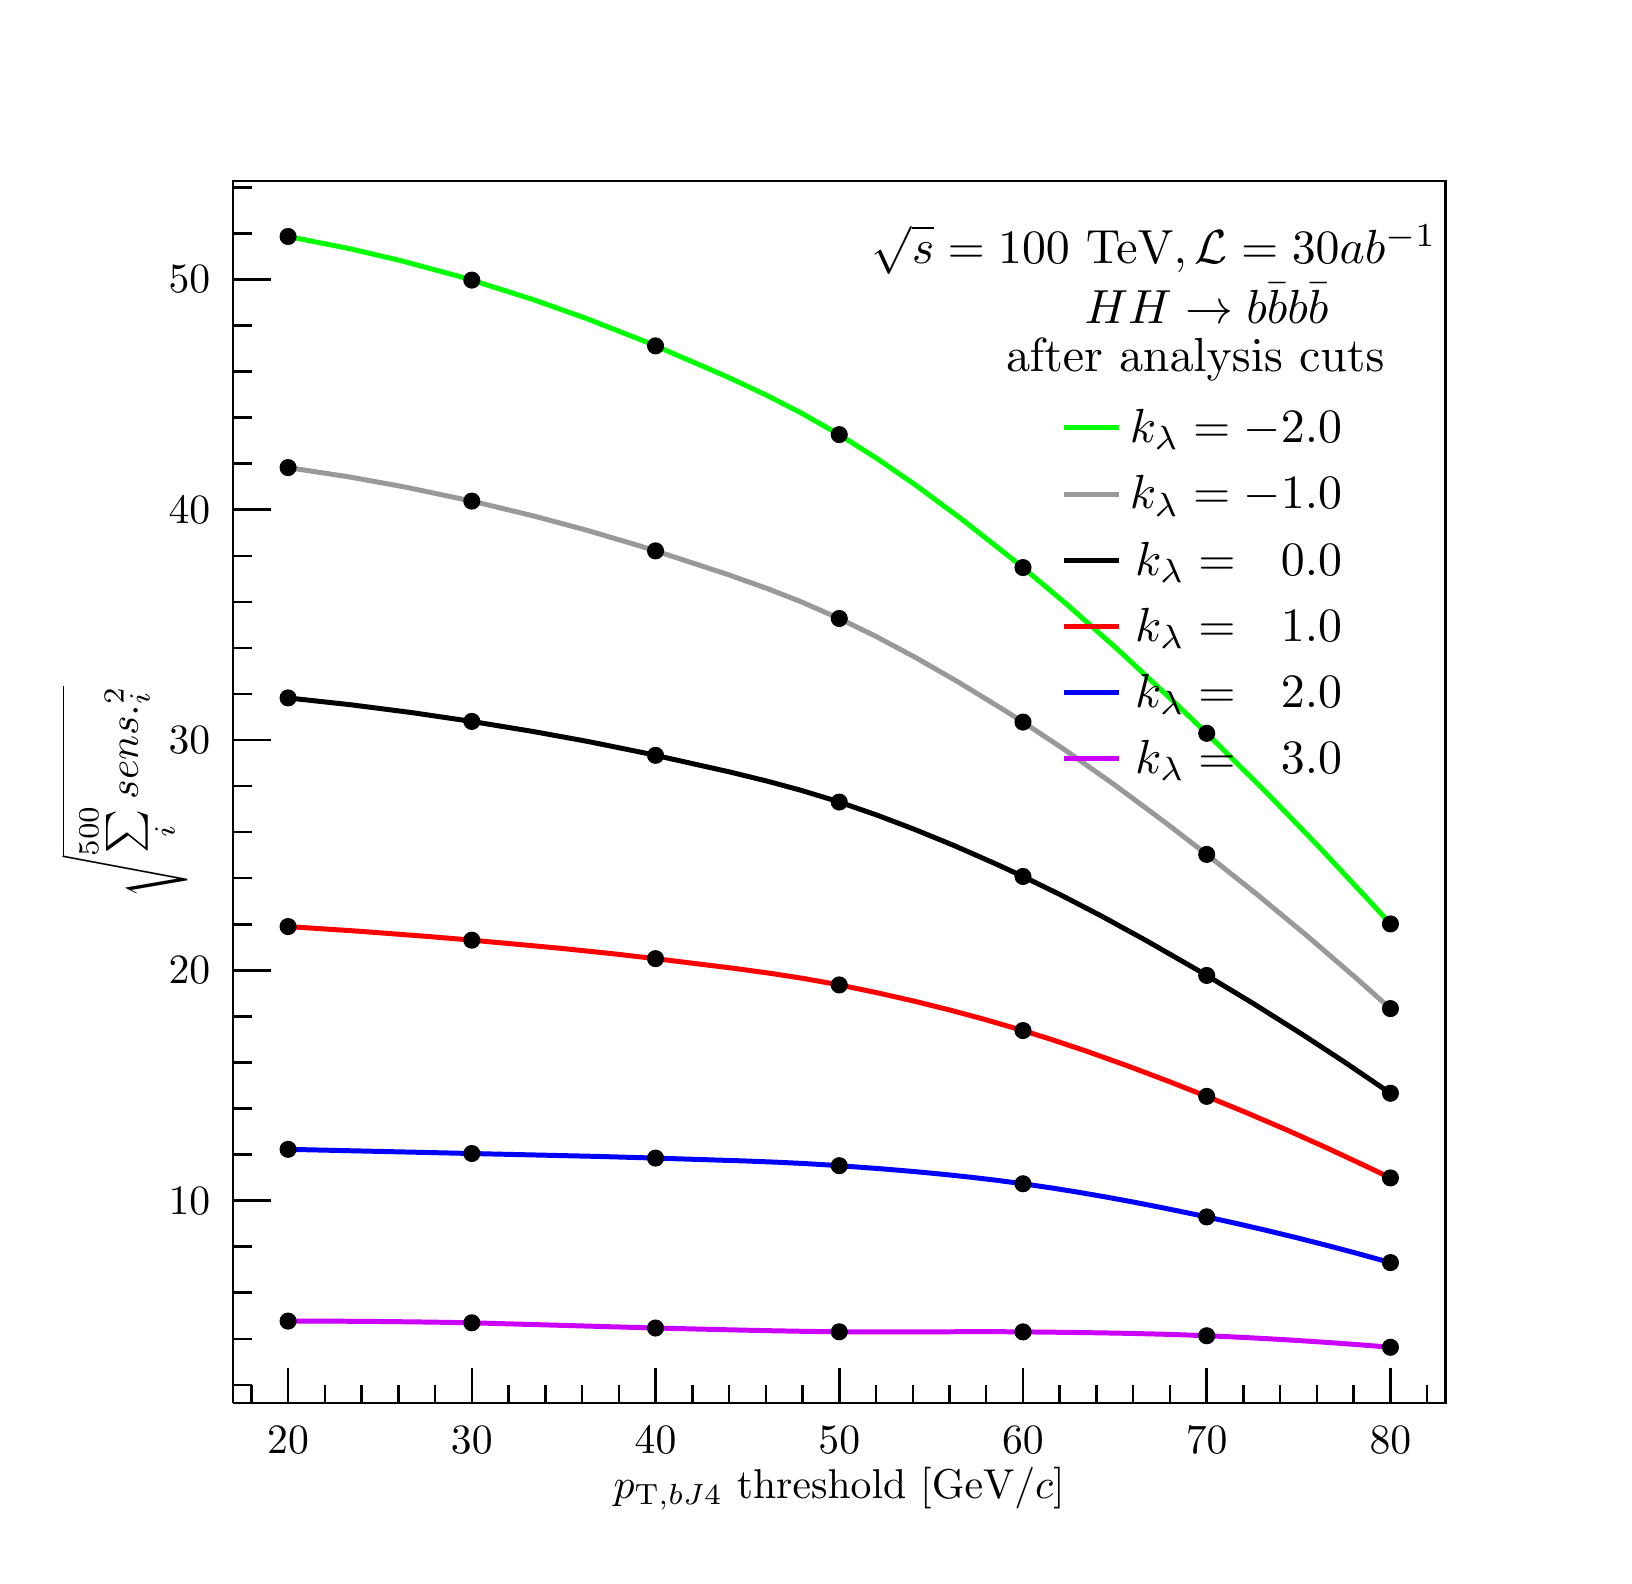
\begin{tikzpicture}
\pgfdeclareplotmark{cross} {
\pgfpathmoveto{\pgfpoint{-0.3\pgfplotmarksize}{\pgfplotmarksize}}
\pgfpathlineto{\pgfpoint{+0.3\pgfplotmarksize}{\pgfplotmarksize}}
\pgfpathlineto{\pgfpoint{+0.3\pgfplotmarksize}{0.3\pgfplotmarksize}}
\pgfpathlineto{\pgfpoint{+1\pgfplotmarksize}{0.3\pgfplotmarksize}}
\pgfpathlineto{\pgfpoint{+1\pgfplotmarksize}{-0.3\pgfplotmarksize}}
\pgfpathlineto{\pgfpoint{+0.3\pgfplotmarksize}{-0.3\pgfplotmarksize}}
\pgfpathlineto{\pgfpoint{+0.3\pgfplotmarksize}{-1.\pgfplotmarksize}}
\pgfpathlineto{\pgfpoint{-0.3\pgfplotmarksize}{-1.\pgfplotmarksize}}
\pgfpathlineto{\pgfpoint{-0.3\pgfplotmarksize}{-0.3\pgfplotmarksize}}
\pgfpathlineto{\pgfpoint{-1.\pgfplotmarksize}{-0.3\pgfplotmarksize}}
\pgfpathlineto{\pgfpoint{-1.\pgfplotmarksize}{0.3\pgfplotmarksize}}
\pgfpathlineto{\pgfpoint{-0.3\pgfplotmarksize}{0.3\pgfplotmarksize}}
\pgfpathclose
\pgfusepathqstroke
}
\pgfdeclareplotmark{cross*} {
\pgfpathmoveto{\pgfpoint{-0.3\pgfplotmarksize}{\pgfplotmarksize}}
\pgfpathlineto{\pgfpoint{+0.3\pgfplotmarksize}{\pgfplotmarksize}}
\pgfpathlineto{\pgfpoint{+0.3\pgfplotmarksize}{0.3\pgfplotmarksize}}
\pgfpathlineto{\pgfpoint{+1\pgfplotmarksize}{0.3\pgfplotmarksize}}
\pgfpathlineto{\pgfpoint{+1\pgfplotmarksize}{-0.3\pgfplotmarksize}}
\pgfpathlineto{\pgfpoint{+0.3\pgfplotmarksize}{-0.3\pgfplotmarksize}}
\pgfpathlineto{\pgfpoint{+0.3\pgfplotmarksize}{-1.\pgfplotmarksize}}
\pgfpathlineto{\pgfpoint{-0.3\pgfplotmarksize}{-1.\pgfplotmarksize}}
\pgfpathlineto{\pgfpoint{-0.3\pgfplotmarksize}{-0.3\pgfplotmarksize}}
\pgfpathlineto{\pgfpoint{-1.\pgfplotmarksize}{-0.3\pgfplotmarksize}}
\pgfpathlineto{\pgfpoint{-1.\pgfplotmarksize}{0.3\pgfplotmarksize}}
\pgfpathlineto{\pgfpoint{-0.3\pgfplotmarksize}{0.3\pgfplotmarksize}}
\pgfpathclose
\pgfusepathqfillstroke
}
\pgfdeclareplotmark{newstar} {
\pgfpathmoveto{\pgfqpoint{0pt}{\pgfplotmarksize}}
\pgfpathlineto{\pgfqpointpolar{44}{0.5\pgfplotmarksize}}
\pgfpathlineto{\pgfqpointpolar{18}{\pgfplotmarksize}}
\pgfpathlineto{\pgfqpointpolar{-20}{0.5\pgfplotmarksize}}
\pgfpathlineto{\pgfqpointpolar{-54}{\pgfplotmarksize}}
\pgfpathlineto{\pgfqpointpolar{-90}{0.5\pgfplotmarksize}}
\pgfpathlineto{\pgfqpointpolar{234}{\pgfplotmarksize}}
\pgfpathlineto{\pgfqpointpolar{198}{0.5\pgfplotmarksize}}
\pgfpathlineto{\pgfqpointpolar{162}{\pgfplotmarksize}}
\pgfpathlineto{\pgfqpointpolar{134}{0.5\pgfplotmarksize}}
\pgfpathclose
\pgfusepathqstroke
}
\pgfdeclareplotmark{newstar*} {
\pgfpathmoveto{\pgfqpoint{0pt}{\pgfplotmarksize}}
\pgfpathlineto{\pgfqpointpolar{44}{0.5\pgfplotmarksize}}
\pgfpathlineto{\pgfqpointpolar{18}{\pgfplotmarksize}}
\pgfpathlineto{\pgfqpointpolar{-20}{0.5\pgfplotmarksize}}
\pgfpathlineto{\pgfqpointpolar{-54}{\pgfplotmarksize}}
\pgfpathlineto{\pgfqpointpolar{-90}{0.5\pgfplotmarksize}}
\pgfpathlineto{\pgfqpointpolar{234}{\pgfplotmarksize}}
\pgfpathlineto{\pgfqpointpolar{198}{0.5\pgfplotmarksize}}
\pgfpathlineto{\pgfqpointpolar{162}{\pgfplotmarksize}}
\pgfpathlineto{\pgfqpointpolar{134}{0.5\pgfplotmarksize}}
\pgfpathclose
\pgfusepathqfillstroke
}
\definecolor{c}{rgb}{1,1,1};
\draw [color=c, fill=c] (0,0) rectangle (20,19.397);
\draw [color=c, fill=c] (2.6,1.9397) rectangle (18,17.4573);
\definecolor{c}{rgb}{0,0,0};
\draw [c,line width=0.9] (2.6,1.9397) -- (2.6,17.4573) -- (18,17.4573) -- (18,1.9397) -- (2.6,1.9397);
\definecolor{c}{rgb}{1,1,1};
\draw [color=c, fill=c] (2.6,1.9397) rectangle (18,17.4573);
\definecolor{c}{rgb}{0,0,0};
\draw [c,line width=0.9] (2.6,1.9397) -- (2.6,17.4573) -- (18,17.4573) -- (18,1.9397) -- (2.6,1.9397);
\definecolor{c}{rgb}{0,0,0.6};
\draw [c,line width=0.9] (2.6,1.9397) -- (2.754,1.9397) -- (2.754,1.9397) -- (2.908,1.9397) -- (2.908,1.9397) -- (3.062,1.9397) -- (3.062,1.9397) -- (3.216,1.9397) -- (3.216,1.9397) -- (3.37,1.9397) -- (3.37,1.9397) -- (3.524,1.9397) --
 (3.524,1.9397) -- (3.678,1.9397) -- (3.678,1.9397) -- (3.832,1.9397) -- (3.832,1.9397) -- (3.986,1.9397) -- (3.986,1.9397) -- (4.14,1.9397) -- (4.14,1.9397) -- (4.294,1.9397) -- (4.294,1.9397) -- (4.448,1.9397) -- (4.448,1.9397) -- (4.602,1.9397) --
 (4.602,1.9397) -- (4.756,1.9397) -- (4.756,1.9397) -- (4.91,1.9397) -- (4.91,1.9397) -- (5.064,1.9397) -- (5.064,1.9397) -- (5.218,1.9397) -- (5.218,1.9397) -- (5.372,1.9397) -- (5.372,1.9397) -- (5.526,1.9397) -- (5.526,1.9397) -- (5.68,1.9397) --
 (5.68,1.9397) -- (5.834,1.9397) -- (5.834,1.9397) -- (5.988,1.9397) -- (5.988,1.9397) -- (6.142,1.9397) -- (6.142,1.9397) -- (6.296,1.9397) -- (6.296,1.9397) -- (6.45,1.9397) -- (6.45,1.9397) -- (6.604,1.9397) -- (6.604,1.9397) -- (6.758,1.9397) --
 (6.758,1.9397) -- (6.912,1.9397) -- (6.912,1.9397) -- (7.066,1.9397) -- (7.066,1.9397) -- (7.22,1.9397) -- (7.22,1.9397) -- (7.374,1.9397) -- (7.374,1.9397) -- (7.528,1.9397) -- (7.528,1.9397) -- (7.682,1.9397) -- (7.682,1.9397) -- (7.836,1.9397) --
 (7.836,1.9397) -- (7.99,1.9397) -- (7.99,1.9397) -- (8.144,1.9397) -- (8.144,1.9397) -- (8.298,1.9397) -- (8.298,1.9397) -- (8.452,1.9397) -- (8.452,1.9397) -- (8.606,1.9397) -- (8.606,1.9397) -- (8.76,1.9397) -- (8.76,1.9397) -- (8.914,1.9397) --
 (8.914,1.9397) -- (9.068,1.9397) -- (9.068,1.9397) -- (9.222,1.9397) -- (9.222,1.9397) -- (9.376,1.9397) -- (9.376,1.9397) -- (9.53,1.9397) -- (9.53,1.9397) -- (9.684,1.9397) -- (9.684,1.9397) -- (9.838,1.9397) -- (9.838,1.9397) -- (9.992,1.9397) --
 (9.992,1.9397) -- (10.146,1.9397) -- (10.146,1.9397) -- (10.3,1.9397) -- (10.3,1.9397) -- (10.454,1.9397) -- (10.454,1.9397) -- (10.608,1.9397) -- (10.608,1.9397) -- (10.762,1.9397) -- (10.762,1.9397) -- (10.916,1.9397) -- (10.916,1.9397) --
 (11.07,1.9397) -- (11.07,1.9397) -- (11.224,1.9397) -- (11.224,1.9397) -- (11.378,1.9397) -- (11.378,1.9397) -- (11.532,1.9397) -- (11.532,1.9397) -- (11.686,1.9397) -- (11.686,1.9397) -- (11.84,1.9397) -- (11.84,1.9397) -- (11.994,1.9397) --
 (11.994,1.9397) -- (12.148,1.9397) -- (12.148,1.9397) -- (12.302,1.9397) -- (12.302,1.9397) -- (12.456,1.9397) -- (12.456,1.9397) -- (12.61,1.9397) -- (12.61,1.9397) -- (12.764,1.9397) -- (12.764,1.9397) -- (12.918,1.9397) -- (12.918,1.9397) --
 (13.072,1.9397) -- (13.072,1.9397) -- (13.226,1.9397) -- (13.226,1.9397) -- (13.38,1.9397) -- (13.38,1.9397) -- (13.534,1.9397) -- (13.534,1.9397) -- (13.688,1.9397) -- (13.688,1.9397) -- (13.842,1.9397) -- (13.842,1.9397) -- (13.996,1.9397) --
 (13.996,1.9397) -- (14.15,1.9397) -- (14.15,1.9397) -- (14.304,1.9397) -- (14.304,1.9397) -- (14.458,1.9397) -- (14.458,1.9397) -- (14.612,1.9397) -- (14.612,1.9397) -- (14.766,1.9397) -- (14.766,1.9397) -- (14.92,1.9397) -- (14.92,1.9397) --
 (15.074,1.9397) -- (15.074,1.9397) -- (15.228,1.9397) -- (15.228,1.9397) -- (15.382,1.9397) -- (15.382,1.9397) -- (15.536,1.9397) -- (15.536,1.9397) -- (15.69,1.9397) -- (15.69,1.9397) -- (15.844,1.9397) -- (15.844,1.9397) -- (15.998,1.9397) --
 (15.998,1.9397) -- (16.152,1.9397) -- (16.152,1.9397) -- (16.306,1.9397) -- (16.306,1.9397) -- (16.46,1.9397) -- (16.46,1.9397) -- (16.614,1.9397) -- (16.614,1.9397) -- (16.768,1.9397) -- (16.768,1.9397) -- (16.922,1.9397) -- (16.922,1.9397) --
 (17.076,1.9397) -- (17.076,1.9397) -- (17.23,1.9397) -- (17.23,1.9397) -- (17.384,1.9397) -- (17.384,1.9397) -- (17.538,1.9397) -- (17.538,1.9397) -- (17.692,1.9397) -- (17.692,1.9397) -- (17.846,1.9397) -- (17.846,1.9397) -- (18,1.9397);
\definecolor{c}{rgb}{0,0,0};
\draw [c,line width=0.9] (2.6,1.9397) -- (18,1.9397);
\draw [c,line width=0.9] (3.3,2.38777) -- (3.3,1.9397);
\draw [c,line width=0.9] (3.76667,2.16373) -- (3.76667,1.9397);
\draw [c,line width=0.9] (4.23333,2.16373) -- (4.23333,1.9397);
\draw [c,line width=0.9] (4.7,2.16373) -- (4.7,1.9397);
\draw [c,line width=0.9] (5.16667,2.16373) -- (5.16667,1.9397);
\draw [c,line width=0.9] (5.63333,2.38777) -- (5.63333,1.9397);
\draw [c,line width=0.9] (6.1,2.16373) -- (6.1,1.9397);
\draw [c,line width=0.9] (6.56667,2.16373) -- (6.56667,1.9397);
\draw [c,line width=0.9] (7.03333,2.16373) -- (7.03333,1.9397);
\draw [c,line width=0.9] (7.5,2.16373) -- (7.5,1.9397);
\draw [c,line width=0.9] (7.96667,2.38777) -- (7.96667,1.9397);
\draw [c,line width=0.9] (8.43333,2.16373) -- (8.43333,1.9397);
\draw [c,line width=0.9] (8.9,2.16373) -- (8.9,1.9397);
\draw [c,line width=0.9] (9.36667,2.16373) -- (9.36667,1.9397);
\draw [c,line width=0.9] (9.83333,2.16373) -- (9.83333,1.9397);
\draw [c,line width=0.9] (10.3,2.38777) -- (10.3,1.9397);
\draw [c,line width=0.9] (10.7667,2.16373) -- (10.7667,1.9397);
\draw [c,line width=0.9] (11.2333,2.16373) -- (11.2333,1.9397);
\draw [c,line width=0.9] (11.7,2.16373) -- (11.7,1.9397);
\draw [c,line width=0.9] (12.1667,2.16373) -- (12.1667,1.9397);
\draw [c,line width=0.9] (12.6333,2.38777) -- (12.6333,1.9397);
\draw [c,line width=0.9] (13.1,2.16373) -- (13.1,1.9397);
\draw [c,line width=0.9] (13.5667,2.16373) -- (13.5667,1.9397);
\draw [c,line width=0.9] (14.0333,2.16373) -- (14.0333,1.9397);
\draw [c,line width=0.9] (14.5,2.16373) -- (14.5,1.9397);
\draw [c,line width=0.9] (14.9667,2.38777) -- (14.9667,1.9397);
\draw [c,line width=0.9] (15.4333,2.16373) -- (15.4333,1.9397);
\draw [c,line width=0.9] (15.9,2.16373) -- (15.9,1.9397);
\draw [c,line width=0.9] (16.3667,2.16373) -- (16.3667,1.9397);
\draw [c,line width=0.9] (16.8333,2.16373) -- (16.8333,1.9397);
\draw [c,line width=0.9] (17.3,2.38777) -- (17.3,1.9397);
\draw [c,line width=0.9] (3.3,2.38777) -- (3.3,1.9397);
\draw [c,line width=0.9] (2.83333,2.16373) -- (2.83333,1.9397);
\draw [c,line width=0.9] (17.3,2.38777) -- (17.3,1.9397);
\draw [c,line width=0.9] (17.7667,2.16373) -- (17.7667,1.9397);
\draw [anchor=base] (3.3,1.2996) node[scale=1.50669, color=c, rotate=0]{20};
\draw [anchor=base] (5.63333,1.2996) node[scale=1.50669, color=c, rotate=0]{30};
\draw [anchor=base] (7.96667,1.2996) node[scale=1.50669, color=c, rotate=0]{40};
\draw [anchor=base] (10.3,1.2996) node[scale=1.50669, color=c, rotate=0]{50};
\draw [anchor=base] (12.6333,1.2996) node[scale=1.50669, color=c, rotate=0]{60};
\draw [anchor=base] (14.9667,1.2996) node[scale=1.50669, color=c, rotate=0]{70};
\draw [anchor=base] (17.3,1.2996) node[scale=1.50669, color=c, rotate=0]{80};
\draw (10.3,0.853467) node[scale=1.50669, color=c, rotate=0]{$p_{\text{T}, bJ4} \text{~threshold} ~[\text{GeV}/c]$};
\draw [c,line width=0.9] (2.6,1.9397) -- (2.6,17.4573);
\draw [c,line width=0.9] (3.08,4.50756) -- (2.6,4.50756);
\draw [c,line width=0.9] (2.84,5.09252) -- (2.6,5.09252);
\draw [c,line width=0.9] (2.84,5.67748) -- (2.6,5.67748);
\draw [c,line width=0.9] (2.84,6.26244) -- (2.6,6.26244);
\draw [c,line width=0.9] (2.84,6.8474) -- (2.6,6.8474);
\draw [c,line width=0.9] (3.08,7.43236) -- (2.6,7.43236);
\draw [c,line width=0.9] (2.84,8.01732) -- (2.6,8.01732);
\draw [c,line width=0.9] (2.84,8.60228) -- (2.6,8.60228);
\draw [c,line width=0.9] (2.84,9.18724) -- (2.6,9.18724);
\draw [c,line width=0.9] (2.84,9.7722) -- (2.6,9.7722);
\draw [c,line width=0.9] (3.08,10.3572) -- (2.6,10.3572);
\draw [c,line width=0.9] (2.84,10.9421) -- (2.6,10.9421);
\draw [c,line width=0.9] (2.84,11.5271) -- (2.6,11.5271);
\draw [c,line width=0.9] (2.84,12.112) -- (2.6,12.112);
\draw [c,line width=0.9] (2.84,12.697) -- (2.6,12.697);
\draw [c,line width=0.9] (3.08,13.282) -- (2.6,13.282);
\draw [c,line width=0.9] (2.84,13.8669) -- (2.6,13.8669);
\draw [c,line width=0.9] (2.84,14.4519) -- (2.6,14.4519);
\draw [c,line width=0.9] (2.84,15.0368) -- (2.6,15.0368);
\draw [c,line width=0.9] (2.84,15.6218) -- (2.6,15.6218);
\draw [c,line width=0.9] (3.08,16.2068) -- (2.6,16.2068);
\draw [c,line width=0.9] (3.08,4.50756) -- (2.6,4.50756);
\draw [c,line width=0.9] (2.84,3.9226) -- (2.6,3.9226);
\draw [c,line width=0.9] (2.84,3.33764) -- (2.6,3.33764);
\draw [c,line width=0.9] (2.84,2.75268) -- (2.6,2.75268);
\draw [c,line width=0.9] (2.84,2.16772) -- (2.6,2.16772);
\draw [c,line width=0.9] (3.08,16.2068) -- (2.6,16.2068);
\draw [c,line width=0.9] (2.84,16.7917) -- (2.6,16.7917);
\draw [c,line width=0.9] (2.84,17.3767) -- (2.6,17.3767);
\draw [anchor= east] (2.5,4.50756) node[scale=1.50669, color=c, rotate=0]{10};
\draw [anchor= east] (2.5,7.43236) node[scale=1.50669, color=c, rotate=0]{20};
\draw [anchor= east] (2.5,10.3572) node[scale=1.50669, color=c, rotate=0]{30};
\draw [anchor= east] (2.5,13.282) node[scale=1.50669, color=c, rotate=0]{40};
\draw [anchor= east] (2.5,16.2068) node[scale=1.50669, color=c, rotate=0]{50};
\draw (1.22161,9.69849) node[scale=1.50669, color=c, rotate=90]{$\sqrt{ \sum\limits_{i}^{500} sens._{i}^{2}}$};
\definecolor{c}{rgb}{0,1,0};
\draw [c,line width=1.8] (3.3,16.7519) -- (4.08293,16.5974) -- (4.76075,16.4381) -- (5.47627,16.2441) -- (5.63333,16.198) -- (6.41376,15.9504) -- (7.07963,15.7143) -- (7.7773,15.4415) -- (7.96667,15.3629) -- (8.86078,14.9777) -- (9.36837,14.7403) --
 (9.80858,14.5152) -- (10.3,14.2359) -- (10.7691,13.9392) -- (11.2764,13.5903) -- (11.8519,13.1645) -- (12.5023,12.6533) -- (12.6333,12.5473) -- (13.1888,12.0819) -- (13.8454,11.4995) -- (14.5446,10.8482) -- (14.9667,10.4427) -- (15.7355,9.67995) --
 (16.3782,9.016) -- (17.0526,8.29337) -- (17.3,8.02165);
\definecolor{c}{rgb}{0,0,0};
\foreach \P in {(3.3,16.7519), (5.63333,16.198), (7.96667,15.3629), (10.3,14.2359), (12.6333,12.5473), (14.9667,10.4427), (17.3,8.02165)}{\draw[mark options={color=c,fill=c},mark size=2.882883pt,mark=*] plot coordinates {\P};}
\definecolor{c}{rgb}{0.6,0.6,0.6};
\draw [c,line width=1.8] (3.3,13.8173) -- (4.09326,13.6956) -- (4.7959,13.5679) -- (5.63333,13.3914) -- (6.41932,13.2023) -- (7.0891,13.0227) -- (7.78318,12.8172) -- (7.96667,12.7593) -- (8.88617,12.4588) -- (9.38384,12.2815) -- (9.81388,12.1132) --
 (10.3,11.9006) -- (10.7691,11.6713) -- (11.2674,11.4059) -- (11.8125,11.093) -- (12.4086,10.7277) -- (12.6333,10.5848) -- (13.1583,10.2368) -- (13.7984,9.78601) -- (14.4454,9.30573) -- (14.9667,8.90459) -- (15.605,8.39651) -- (16.2337,7.87581) --
 (16.8564,7.34003) -- (17.3,6.94633);
\definecolor{c}{rgb}{0,0,0};
\foreach \P in {(3.3,13.8173), (5.63333,13.3914), (7.96667,12.7593), (10.3,11.9006), (12.6333,10.5848), (14.9667,8.90459), (17.3,6.94633)}{\draw[mark options={color=c,fill=c},mark size=2.882883pt,mark=*] plot coordinates {\P};}
\draw [c,line width=1.8] (3.3,10.8918) -- (4.11554,10.8025) -- (4.86964,10.7056) -- (5.63333,10.5933) -- (6.42975,10.4622) -- (7.10569,10.339) -- (7.79329,10.1999) -- (7.96667,10.1624) -- (8.91788,9.94949) -- (9.40187,9.83057) -- (9.81672,9.71779) --
 (10.2301,9.5921) -- (10.3,9.56929) -- (10.7696,9.40672) -- (11.2547,9.22313) -- (11.7666,9.01329) -- (12.2879,8.78404) -- (12.6333,8.62407) -- (13.1158,8.38856) -- (13.6329,8.12004) -- (14.2066,7.80553) -- (14.8483,7.43686) -- (14.9667,7.36728) --
 (15.5559,7.01207) -- (16.1644,6.6292) -- (16.7252,6.2619) -- (17.3,5.87101);
\foreach \P in {(3.3,10.8918), (5.63333,10.5933), (7.96667,10.1624), (10.3,9.56929), (12.6333,8.62407), (14.9667,7.36728), (17.3,5.87101)}{\draw[mark options={color=c,fill=c},mark size=2.882883pt,mark=*] plot coordinates {\P};}
\definecolor{c}{rgb}{1,0,0};
\draw [c,line width=1.8] (3.3,7.988) -- (4.19137,7.92942) -- (5.09628,7.86066) -- (5.63333,7.81541) -- (6.75067,7.71287) -- (7.4305,7.64247) -- (7.96667,7.58049) -- (8.98368,7.45504) -- (9.44184,7.39178) -- (9.83115,7.33117) -- (10.2198,7.26224) --
 (10.3,7.24678) -- (10.7727,7.14941) -- (11.236,7.04434) -- (11.715,6.92541) -- (12.1424,6.81027) -- (12.6333,6.66728) -- (12.9972,6.55326) -- (13.4436,6.40395) -- (13.977,6.21346) -- (14.4997,6.0158) -- (14.9667,5.83166) -- (15.4782,5.62173) --
 (15.9902,5.40195) -- (16.4887,5.1787) -- (16.993,4.94346) -- (17.3,4.79569);
\definecolor{c}{rgb}{0,0,0};
\foreach \P in {(3.3,7.988), (5.63333,7.81541), (7.96667,7.58049), (10.3,7.24678), (12.6333,6.66728), (14.9667,5.83166), (17.3,4.79569)}{\draw[mark options={color=c,fill=c},mark size=2.882883pt,mark=*] plot coordinates {\P};}
\definecolor{c}{rgb}{0,0,1};
\draw [c,line width=1.8] (3.3,5.159) -- (5.63333,5.10569) -- (7.27317,5.06785) -- (7.96667,5.04765) -- (9.11537,5.01089) -- (9.52354,4.99472) -- (9.86616,4.97805) -- (10.2091,4.95758) -- (10.3,4.95141) -- (10.8386,4.91141) -- (11.2556,4.87631) --
 (11.6365,4.8402) -- (11.9836,4.80324) -- (12.2927,4.76662) -- (12.6333,4.72171) -- (12.9924,4.66907) -- (13.2986,4.62024) -- (13.6545,4.55923) -- (14.0259,4.49108) -- (14.4121,4.41576) -- (14.8296,4.32975) -- (14.9667,4.30058) -- (15.3263,4.22157)
 -- (15.7157,4.13173) -- (16.1026,4.03808) -- (16.5123,3.93412) -- (16.8785,3.83704) -- (17.3,3.72036);
\definecolor{c}{rgb}{0,0,0};
\foreach \P in {(3.3,5.159), (5.63333,5.10569), (7.96667,5.04765), (10.3,4.95141), (12.6333,4.72171), (14.9667,4.30058), (17.3,3.72036)}{\draw[mark options={color=c,fill=c},mark size=2.882883pt,mark=*] plot coordinates {\P};}
\definecolor{c}{rgb}{0.8,0,1};
\draw [c,line width=1.8] (3.3,2.97776) -- (3.65814,2.97726) -- (3.96306,2.97602) -- (4.31284,2.97366) -- (4.66508,2.97028) -- (5.01647,2.96591) -- (5.35706,2.96072) -- (5.63333,2.95581) -- (7.96667,2.88958) -- (8.99215,2.8647) -- (9.40979,2.85567) --
 (9.72291,2.84977) -- (9.99944,2.84537) -- (10.3,2.84162) -- (10.5078,2.83997) -- (10.746,2.83921) -- (11.0399,2.83949) -- (11.5363,2.84151) -- (11.962,2.84303) -- (12.1985,2.8431) -- (12.4043,2.84242) -- (12.6333,2.84061) -- (13.1847,2.83436) --
 (13.5362,2.8295) -- (13.8294,2.82449) -- (14.0833,2.81923) -- (14.3192,2.81339) -- (14.5412,2.80692) -- (14.7348,2.80041) -- (14.9341,2.79277) -- (14.9667,2.79143) -- (15.2025,2.78108) -- (15.4404,2.76965) -- (15.6779,2.75721) -- (15.9275,2.74306)
 -- (16.1397,2.73014) -- (16.3785,2.71463) -- (16.6153,2.69823) -- (16.8569,2.68044) -- (17.0826,2.66287) -- (17.3,2.64504);
\definecolor{c}{rgb}{0,0,0};
\foreach \P in {(3.3,2.97776), (5.63333,2.95581), (7.96667,2.88958), (10.3,2.84162), (12.6333,2.84061), (14.9667,2.79143), (17.3,2.64504)}{\draw[mark options={color=c,fill=c},mark size=2.882883pt,mark=*] plot coordinates {\P};}
\draw [anchor= west] (10.5,16.5844) node[scale=1.7299, color=c, rotate=0]{$\sqrt{s} = 100 ~\text{TeV}, \mathcal{L} = 30 ab^{-1}$};
\draw [anchor= west] (13.2,15.9055) node[scale=1.7299, color=c, rotate=0]{$HH \rightarrow b\bar{b}b\bar{b}$};
\draw [anchor=base west] (12.2,15.0424) node[scale=1.7299, color=c, rotate=0]{after analysis cuts};
\draw [anchor=base east] (16.9,14.1323) node[scale=1.7299, color=c, rotate=0]{$k_{\lambda} = -2.0$};
\definecolor{c}{rgb}{0,1,0};
\draw [c,line width=1.8] (13.15,14.3214) -- (13.85,14.3214);
\definecolor{c}{rgb}{0,0,0};
\draw [anchor=base east] (16.9,13.2918) node[scale=1.7299, color=c, rotate=0]{$k_{\lambda} = -1.0$};
\definecolor{c}{rgb}{0.6,0.6,0.6};
\draw [c,line width=1.8] (13.15,13.4809) -- (13.85,13.4809);
\definecolor{c}{rgb}{0,0,0};
\draw [anchor=base east] (16.9,12.4512) node[scale=1.7299, color=c, rotate=0]{$k_{\lambda} =~~0.0$};
\draw [c,line width=1.8] (13.15,12.6404) -- (13.85,12.6404);
\draw [anchor=base east] (16.9,11.6107) node[scale=1.7299, color=c, rotate=0]{$k_{\lambda} =~~1.0$};
\definecolor{c}{rgb}{1,0,0};
\draw [c,line width=1.8] (13.15,11.7998) -- (13.85,11.7998);
\definecolor{c}{rgb}{0,0,0};
\draw [anchor=base east] (16.9,10.7702) node[scale=1.7299, color=c, rotate=0]{$k_{\lambda} =~~2.0$};
\definecolor{c}{rgb}{0,0,1};
\draw [c,line width=1.8] (13.15,10.9593) -- (13.85,10.9593);
\definecolor{c}{rgb}{0,0,0};
\draw [anchor=base east] (16.9,9.92964) node[scale=1.7299, color=c, rotate=0]{$k_{\lambda} =~~3.0$};
\definecolor{c}{rgb}{0.8,0,1};
\draw [c,line width=1.8] (13.15,10.1188) -- (13.85,10.1188);
\end{tikzpicture}
% end document
\end{document}
